 \documentclass{article}
\usepackage[utf8]{inputenc}
\usepackage{float}
\usepackage{amsmath}
\usepackage[labelsep=period]{caption} % Figur. istället för Figur:
\usepackage{relsize}
\usepackage{multirow}
\usepackage[export]{adjustbox}
\usepackage{subcaption}
\usepackage{wrapfig}
\usepackage{hyperref}
\usepackage{array}
\usepackage{amsmath}
\usepackage{geometry}
\usepackage{parskip}
\newcommand\tab[1][1cm]{\hspace*{#1}}

\title{Reinforcement Learning EL2805\\
       Laboration 1}

\author{Ilian Corenliussen, 950418-2438, ilianc@kth.se\\ 
        Daniel Hirsch, 960202-5737, dhirsch@kth.se}
\date{November 2020}

\begin{document}

\maketitle

\section*{Problem 1: \\
        The Maze and the Random Minotaur}
\subsection*{A)}
The problem can me modelled as an MDP such that, the number of states is depending on the grid space and the player and Minotaur position, e.g. $S = \{((P_x, H_y),(P_x, M_y) )\} $ where $P_x$ and $P_y$ is the player and $M_x$ and $M_y$ the Minotaur position x and y position within the grid. The state space can be divided into $S = {S_a, S_u}$ where $S_a$ is the allowed states and $S_u$ is the unreachable states, such as wall or out-of-boundary.


\textbf{State space:}\\
$S = \{((P_x, H_y),(P_x, M_y) )\} $, 3136 number of states. 

\textbf{Actions}: \\
The actions can be as described in the lab instructions as left, right, up, down or stay at the current position, $A = \{ A_{left}, A_{right}, A_{up}, A_{down}, A_{stay} \}$. 

\textbf{Rewards:} \\
Eaten: $r(P_x = M_x , P_y = M_y |s,a) = -100 $\\ 
Goal: $r(P_x = B_x , P_y = B_y |s,a) = 0 $, where $B_x$, $B_y$ is the goal position\\
Wall: $r(s'\in S_u |s,a) = -\infty $\\
Walking: $r(s'\in S_a |s,a) = -1 $

\textbf{Transition Probabilities}:\\
$P_t(s' \in S_a |s,a) = 1/n$, where n is the number of possible moves for the Minotaur and \\$P_t(s \in S_u |s,a) = 0$. 

\subsection*{B)}
\begin{figure}[H]
    \centering
    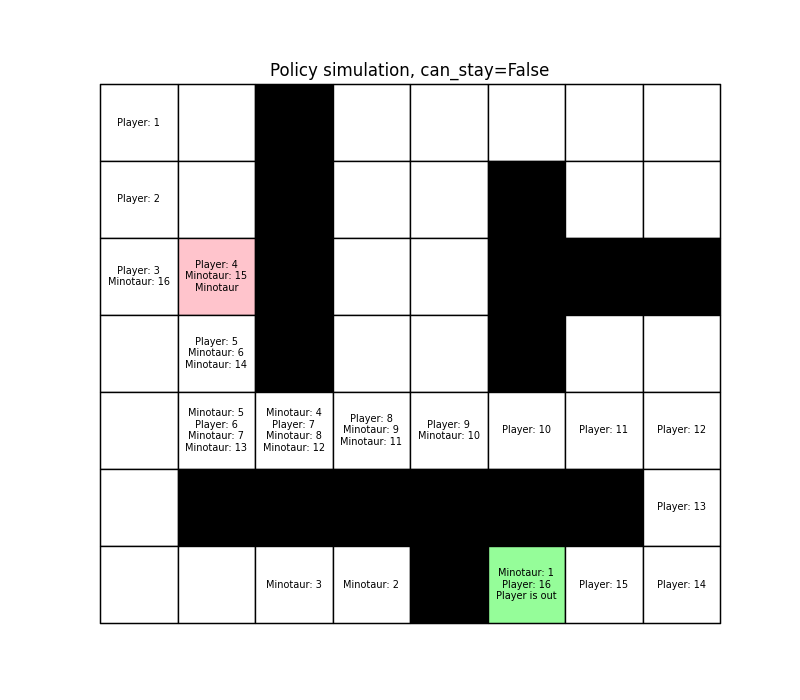
\includegraphics[width=0.8\textwidth]{Lab_1/images/problem_1/MazeRun_Nov-16-2020_10-00-04.png}
    \caption{\small Illustration of the policy for one run, where Player: 1 and Minotaur: 1 is the position for time t=1, etc. }
    \label{fig:Policy}
\end{figure}

\begin{figure}[H]
    \centering
    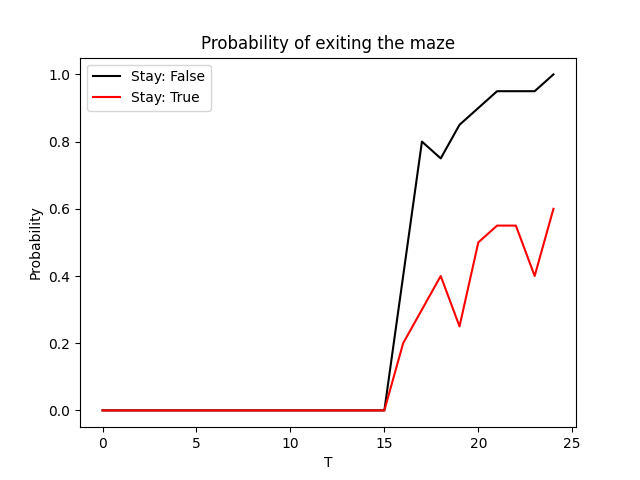
\includegraphics[width=0.8\textwidth]{Lab_1/images/problem_1/probability_of_exiting_the_maze_2.png}
    \caption{\small Probability of exiting the maze as a function of T, with 20 runs for each $t=1,2,3,...,25$.}
    \label{fig:probability_exiting}
\end{figure}

\end{document}
